\documentclass[conference]{IEEEtran}

\ifCLASSINFOpdf
   \usepackage[pdftex]{graphicx}
  % declare the path(s) where your graphic files are
   \graphicspath{{../pdf/}{../jpeg/}}
  % and their extensions so you won't have to specify these with
  % every instance of \includegraphics
   \DeclareGraphicsExtensions{.pdf,.jpeg,.png}
\else
  % or other class option (dvipsone, dvipdf, if not using dvips). graphicx
  % will default to the driver specified in the system graphics.cfg if no
  % driver is specified.
  \usepackage[dvips]{graphicx}
  % declare the path(s) where your graphic files are
  \graphicspath{{../eps/}}
  % and their extensions so you won't have to specify these with
  % every instance of \includegraphics
  \DeclareGraphicsExtensions{.eps}
\fi


\usepackage[utf8x]{inputenc}
\usepackage[T1]{fontenc}
\usepackage{lmodern}
\usepackage{booktabs}
\usepackage{multirow}
\usepackage{algorithmic}
\usepackage[Algoritmo]{algorithm}
\usepackage[spanish,USenglish]{babel}
\usepackage[colorlinks=true,linkcolor=black,urlcolor=black,citecolor=black, urlcolor=black, filecolor=black bookmarks=false]{hyperref}
\usepackage{subfigure}


\addto\captionsspanish{
 \def\tablename{Tabla}}


\begin{document}

\pagestyle{empty}  

\selectlanguage{spanish}

\title{Wind}

\author{\IEEEauthorblockN{GIEE}
\IEEEauthorblockA{Universidad de Nariño\\
San Juan de Pasto, Colombia\\
Email: }
\and
\IEEEauthorblockN{GIIWW}
\IEEEauthorblockA{Universidad de Nariño\\
San Juan de Pasto, Colombia\\
Email: }
}

\maketitle

\selectlanguage{USenglish}
\begin{abstract}

En este artículo se presentan los componentes de una investigación orientada
 a analizar los datos de series de tiempo que provee 3TIER viento recopiladas desde
 el año 1980 hasta 2015 en el departamento de Nariño (Colombia) con el objetivo
 de descubrir patrones secuenciales en el comportamiento de la velocidad
 y dirección del viento.
 Se busca poder predecir con suficiente anticipación anomalías en el incremento
 o disminución de estas características para contribuir en la identificación
 de las ubicaciones más idóneas para la implementación de una futura solución
 eólica como alternativa energética.
\end{abstract}
 
\selectlanguage{spanish}


\begin{IEEEkeywords}
wind, time series 
\end{IEEEkeywords}

\thispagestyle{empty} 

\IEEEpeerreviewmaketitle


%\section{Introducción}

\IEEEPARstart Según estudios del Ministerio de Minas y Energía de Colombia, en el departamento de Nariño hay 15 municipios con cobertura eléctrica inferior al 80\% \cite{ministerio_de_minas_y_energia_plan_2008}. Como nueva estratégia para enfrentar esta problemática se ha planteado la medición y estimación de potenciales energéticos en las zonas más viables de la región. Uno de los componentes a analizar es el potencial de biomasa para la generación eléctrica. Sin embargo, uno de los problemas que se plantea para la ubicación de lugares propicios es la ausencia de bases de datos actualizadas en el área de estudio que permitan su respectivo análisis.

Diversas investigaciones han demostrado la utilidad del uso de imágenes satelitales para la generación de modelos que permitan calcular la cantidad de biomasa presente en un determinado lugar. Desde hace más de 30 años, se cuenta con libre acceso al repositorio de imágenes satelitales Landsat \cite{landsat} que con el debido tratamiento pueden ser usadas para calcular valores nominales de biomasa. Sin embargo, dichos modelos requieren la ejecución de trabajo de campo en la zona para inferir fórmulas iniciales a partir de la medición tradicional de una muestra. Dadas las dificultades para realizar dicho trabajo de campo se utilizó imágenes provistas por investigaciones anteriores \cite{baccini2008afirst}, \cite{baccini_estimated_2012} donde se proporciona niveles de biomasa a nivel pan-tropical.  El acceso a imágenes para cada uno de los países tomados en cuenta para el estudio están disponibles en \cite{WHRC}.

Esta investigación esta orientada a cumplir con los requerimientos necesarios para la generación de un modelo de predicción de biomasa y su extrapolación al resto del área de estudio.


El area de estudio de esta investigación fue el departamento de Nariño (Colombia)
el cual esta ubicado en el extremo sur occidental de Colombia, en la frontera con 
Ecuador con una extensión aproximada de 33.268 km, una población de 1,702 millones según
el censo de 2013, su ubicación 
esta en latitud 00° 31' 08'' y 02° 41' 08'' Norte, Longitud 76° 51' 19'' y 79° 01' 34'' Oeste.

\begin{figure}
  \centering
  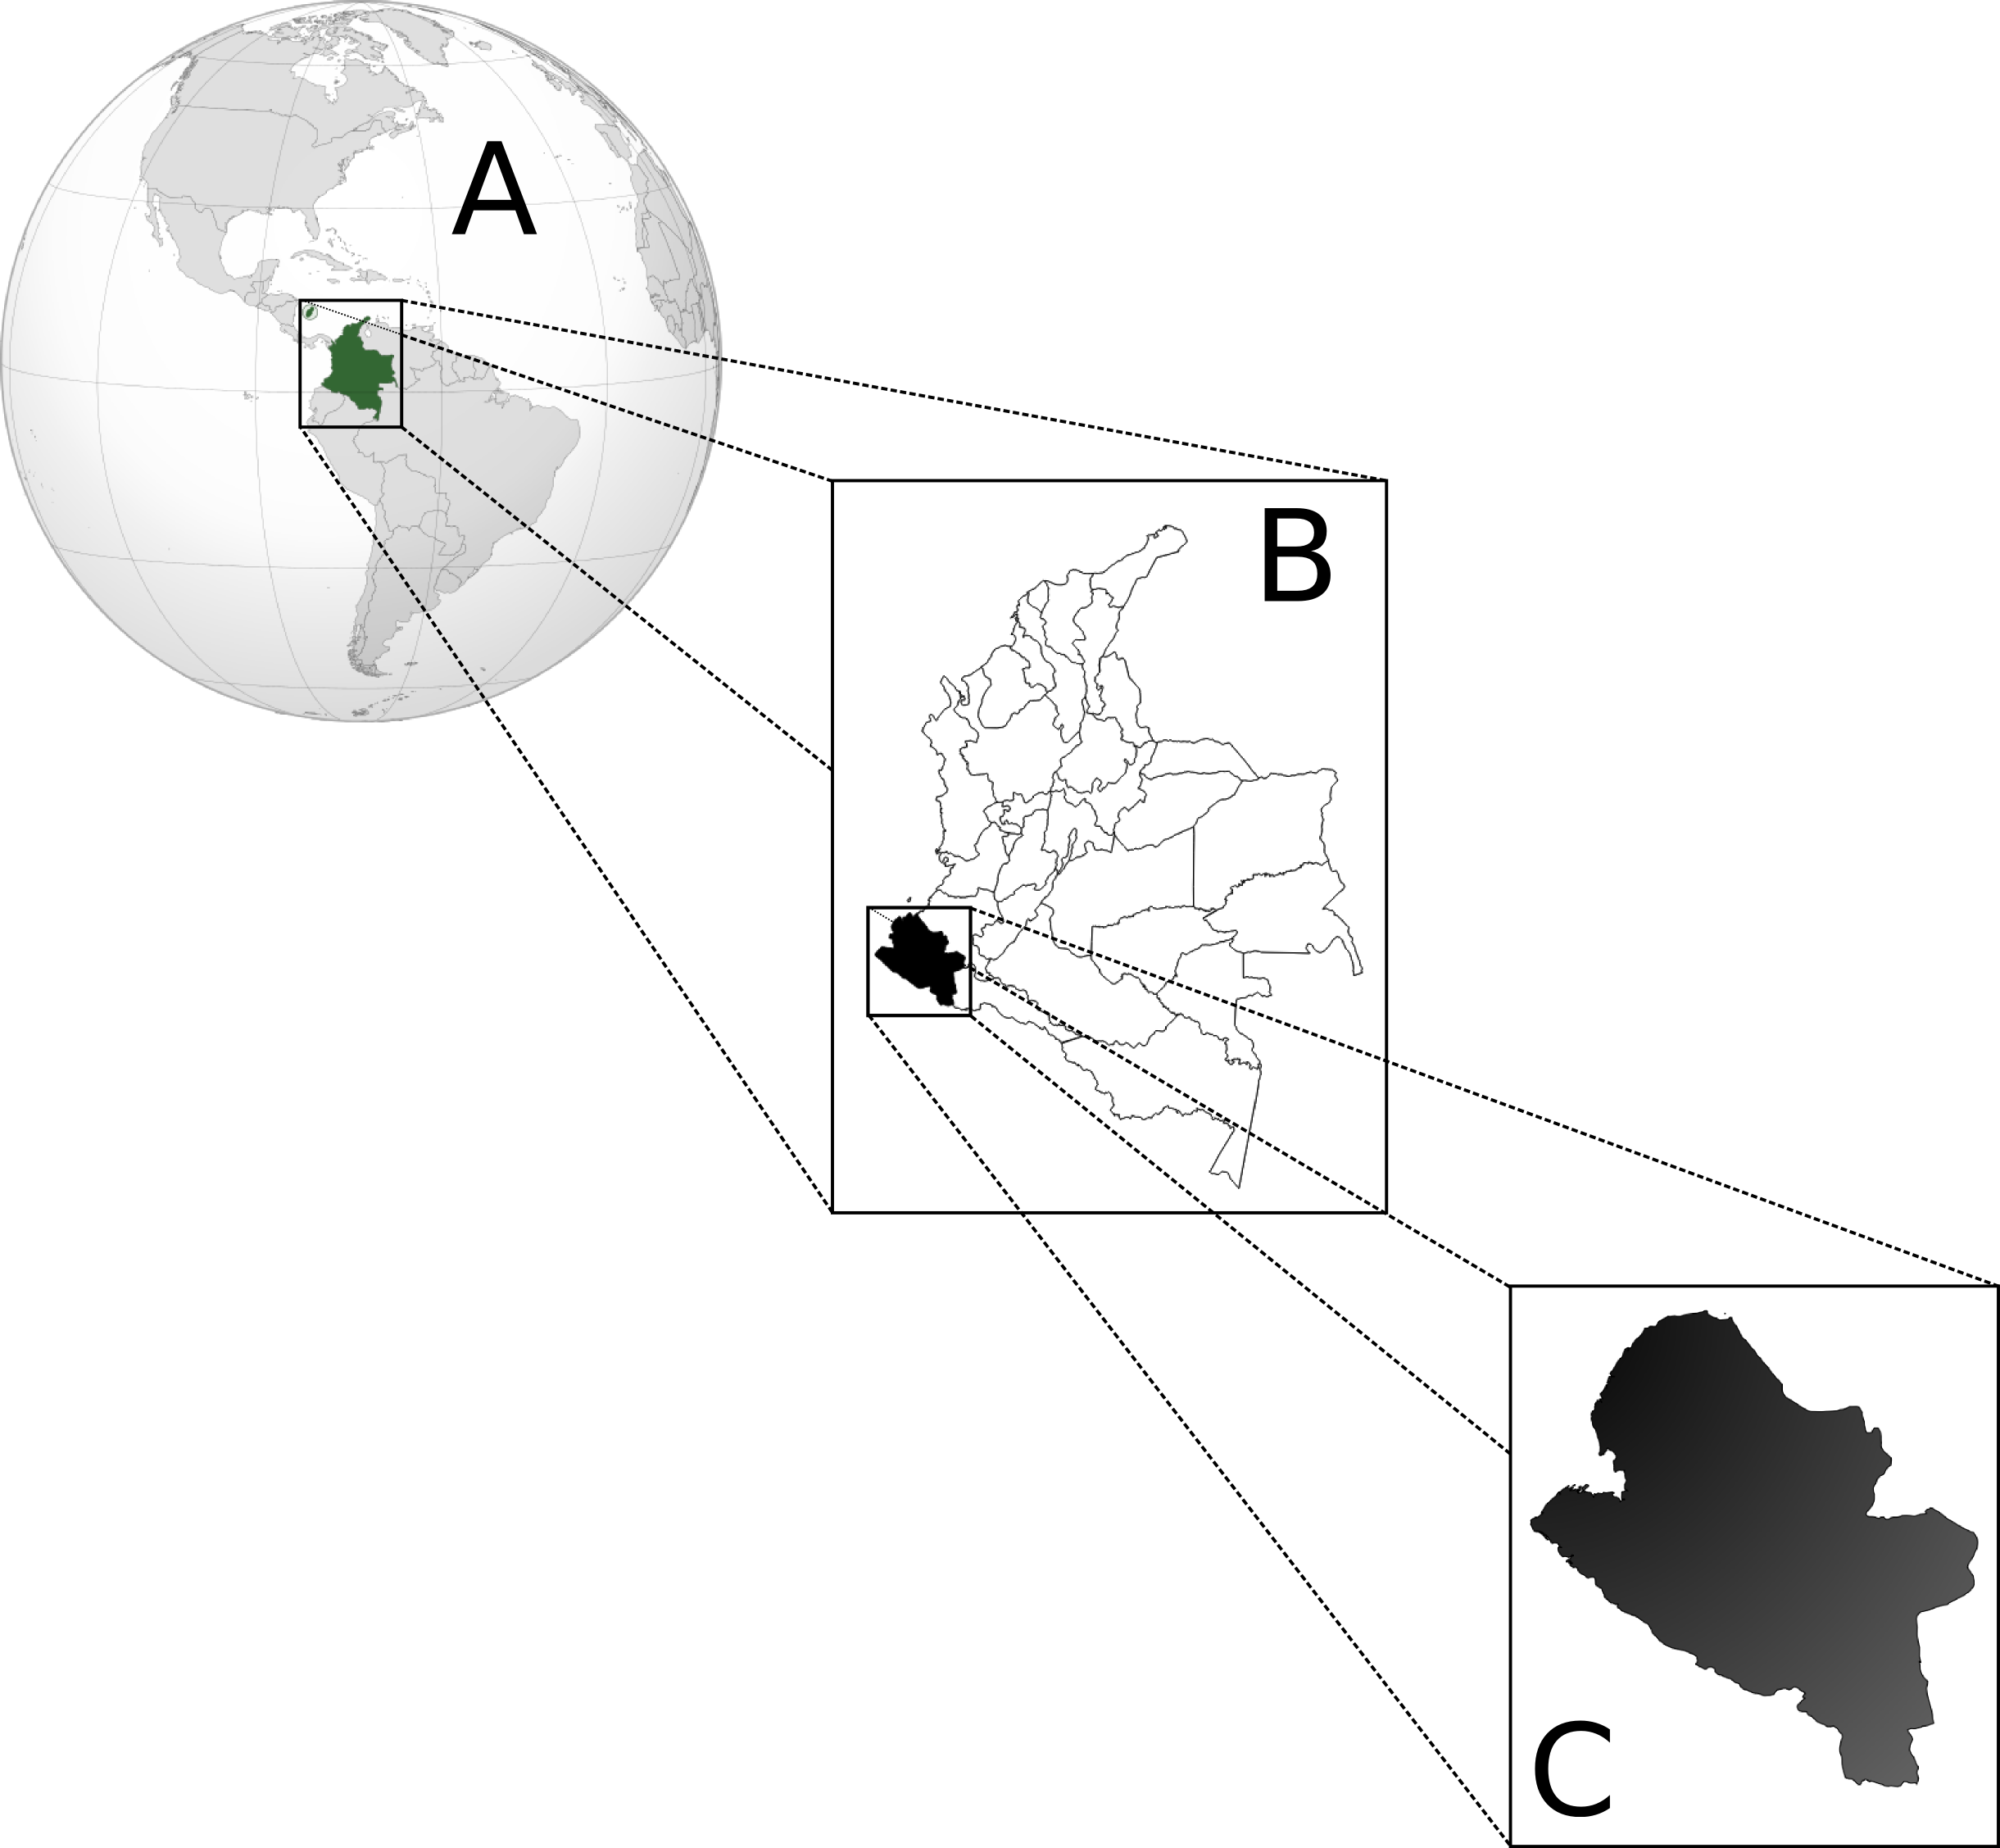
\includegraphics[width = 8cm]{locationNarino.png}
  \caption{Localización area de estudio}
  \label{fig:locationNarino}
\end{figure}
\section{Trabajos relacionados}

Diferentes estudios han explorado la construcción de mapas eólicos a partir
 de muestras tomadas en terreno.
 Por ejemplo, \cite{haslett1989spacetime} utilizan técnicas de auto-correlación espacio-temporal, para estimar la
 potencia generada por turbinas en Irlanda a partir de pocos datos de entrada.
 Adicionales técnicas de interpolación espacial fueron utilizadas por \cite{luo2008acomparison} 
 para generar mapas de viento de alta resolución en el Reino Unido.
 El objetivo perseguido por la investigación era comparar y evaluar diversos
 métodos de interpolación para seleccionar el más adecuado.
 En los Países Bajos, \cite{stepek2011interpolating}  utilizan un modelo llamado de bicapa para estimar la velocidad del viento
 a partir de 31 estaciones meteorológicas.

Sin embargo, es importante resaltar que las características de velocidad
 y dirección del viento no son lo únicos criterios a tener en cuenta a la
 hora de escoger las mejore ubicaciones.
 La evaluación multi-criterio (MCE) ha tenido una amplia acogida a la hora
 de evaluar características físicas junto con otros atributos como aspectos
 económicos y sociales.
 
\cite{rodman2006ageographic}  utilizan técnicas MCE para determinar posibles ubicaciones de turbinas
 en el norte de California evaluando componentes físicos,ambientales y humanos. \cite{janke2010multicriteria}
 categoriza diferentes aspectos de acuerdo al potencial eólico y solar e
 identifica áreas susceptibles a la instalación de turbinas y paneles solares
 en Colorado.
 
 Entre los aspectos evaluados se encuentran la distancia a carreteras y
 líneas de transmisión eléctrica, coberturas del terreno, densidad de población
 y áreas protegidas por la ley. \cite{petrov2014utilization} explora nuevos algoritmos de análisis de datos para modelar la ubicación
 de turbinas en Iowa apoyándose en un sistema espacial multi-criterio de
 soporte a la toma de decisiones.
 Nuevas técnicas de análisis de datos, comúnmente conocidas como minería
 de datos, han demostrado muy buenos resultados a la hora de modelar fenómenos
 atmosféricos.
 
 Por ejemplo, \cite{yusof2014miningfrequent} utiliza algoritmos para detectar patrones secuenciales en series de tiempo
 de viento desde estaciones en los Países Bajos para detectar anomalías
 en el flujo, velocidad y dirección del viento.




%\appendices
%\section{Repositorio}
%El código fuente y conjunto de datos se encuentran en el repositorio de github.


\ifCLASSOPTIONcompsoc
  % The Computer Society usually uses the plural form
  \section*{Agradecimientos}
\else
  % regular IEEE prefers the singular form
  \section*{Agradecimientos}
\fi

Universidad de Nariño, Universidad de los Andes y Sistema de Regalias.

% Can use something like this to put references on a page
% by themselves when using endfloat and the captionsoff option.
\ifCLASSOPTIONcaptionsoff
  \newpage
\fi


\bibliographystyle{IEEEtran}

\bibliography{IEEEabrv,bibliography}



\end{document}
